\documentclass[letterpaper]{article}

\usepackage[utf8]{inputenc}

\usepackage{listings}
\usepackage{color}
\usepackage{graphicx}
    
%New colors defined below
\definecolor{codegreen}{rgb}{0,0.6,0}
\definecolor{codegray}{rgb}{0.5,0.5,0.5}
\definecolor{codepurple}{rgb}{0.58,0,0.90}
\definecolor{backcolour}{rgb}{0.95,0.95,0.92}

%Code listing style named "mystyle"
\lstdefinestyle{mystyle}{
  backgroundcolor=\color{backcolour},   commentstyle=\color{codegreen},
  keywordstyle=\color{magenta},
  numberstyle=\tiny\color{codegray},
  stringstyle=\color{codepurple},
  basicstyle=\footnotesize,
  breakatwhitespace=false,         
  breaklines=true,                 
  captionpos=b,                    
  keepspaces=true,                 
  %numbers=false,                    
  numbersep=5pt,                  
  showspaces=false,                
  showstringspaces=false,
  showtabs=false,                  
  tabsize=2
}

%"mystyle" code listing set
\lstset{style=mystyle}

\usepackage[letterpaper,margin=1.75in,noheadfoot]{geometry}
\usepackage{fontspec, color, enumerate, sectsty}
\usepackage[normalem]{ulem}
\usepackage{amsmath}
\usepackage{listings}

\newcommand{\reporttitle}{An Introduction to Git}
\newcommand{\name}{By Shiva Bhusal}
\newcommand{\course}{}

\usepackage[bookmarks, colorlinks, breaklinks,
pdftitle={\name - \reporttitle},pdfauthor={\name}, unicode]{hyperref}

\hypersetup{
    colorlinks=true,
    linkcolor=blue,
    filecolor=magenta,      
    urlcolor=cyan,
    pdftitle={Sharelatex Example},
    bookmarks=true,
    pdfpagemode=FullScreen,
    }

\usepackage{hyperref}


%%% Start of our document 

\begin{document}
\begin{center}{\huge \scshape \reporttitle}\end{center}
\begin{center}\vspace{0.2em} {\Large \name\\}
  {\course}\end{center} 
  
\tableofcontents
  
\section{Introduction}
\textit{Git} is a distributed version control system which can serve as a better alternative to centralized version control systems like \textit{TFS} and \textit{SVN}. There are many advantages of \textit{Git} over the centralized version control systems which can be summarized in the following points:
\begin{itemize}
    \item It is distributed. So, each developer has a full copy of the repository.
    \item It handles complex merges faster.
    \item For collaborative development involving thousands of developers, \textit{Git} suits better than centralized version control systems.
    \item Branching is cheap and switching between branches is easy.
    \item In general, it provides more functionality and control than the centralized version control systems.
\end{itemize}

Besides, most of the open source projects use \textit{Git} as the version control system. So, if you are interested in open source contribution, you are expected to know the basics of \textit{Git}. In this tutorial, you will learn how to install and setup \textit{Git} and use it as a version control system for your projects. 

\section{Installation and Setup}
    Follow the instructions in the link below to download and install \textit{Git}.\\

%\begin{lstlisting}[language=Bash]
\url{https://git-scm.com/downloads}
%\end{lstlisting}
\\

After you install \textit{Git}, create an account on \href{https://github.com/}{\textit{Github}} or \href{https://about.gitlab.com/}{\textit{Gitlab}}.
Then, set up your identity using the commands below.\\

\begin{lstlisting}[language=Bash]
git config --global user.name "Jane Doe"
git config --global user.email "jane.doe@gmail.com"
\end{lstlisting}

This will make sure that every time you make an update and push it, you are listed as the author of that update.\\

\section{Creating Repository}
This tutorial is based on the assumption that you are using \textit{Github} or \textit{Gitlab}.To get started, create a repository in \textit{Github} or \textit{Gitlab} using the web browser. \\

Alternatively, you can also use \textit{git init} command to create a repository in your local machine. You can learn more about \textit{git init} in the \href{https://git-scm.com/docs/git-init}{\textit{Git} Documentation}

\section{Basic Git Commands}
\subsection{git clone}
It creates a replica of the specified repository. In the example below, the command replicates the repository named \textit{git-demo}.

 \begin{figure}[h]
    \centering
    \frame{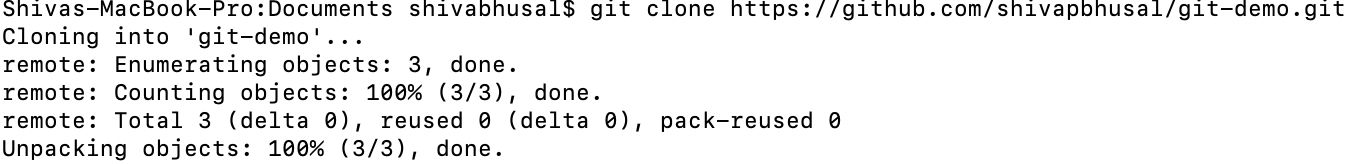
\includegraphics[scale=0.56]{figure/clone.png}}
    \caption{Cloning repository \textit{git-demo}}
  \end{figure}

\subsection{git status}
It displays the current status of the files in the local repository. The example below shows that there is an un-tracked file called \textit{foo.py}.

\begin{figure}[h]
    \centering
    \frame{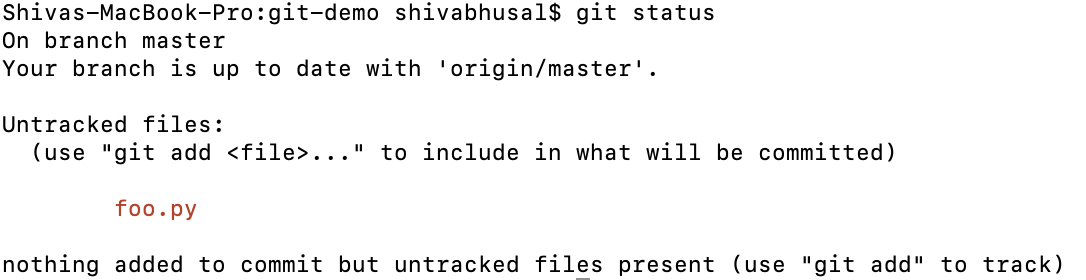
\includegraphics[scale=0.7]{figure/status.png}}
    \caption{\textit{git status} after creating \textit{foo.py}}
  \end{figure}


\subsection{git add}
This command adds the changes for staging. In other words, it marks the specified changes in the current version of the repository which will go into the next version. For example, to add the un-tracked file, \textit{foo.py}, you can use the command below.
\begin{lstlisting}[language=Bash]
git add foo.py
\end{lstlisting}

\subsection{git commit}
 After \textit{git commit}, a new version of the local repository is created which consists of all the changes added.

\begin{figure}[h]
    \centering
    \frame{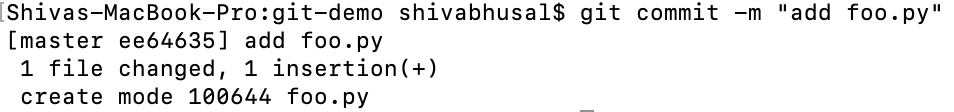
\includegraphics[scale=0.8]{figure/commit.png}}
    \caption{\textit{git commit} operation}
  \end{figure}


\subsection{git push}
It merges the locally committed changes with the repository in the remote server.

\begin{lstlisting}[language=Bash]
git push
\end{lstlisting}


\subsection{git pull}
Suppose, another member of the team has already pushed the changes. In such situations, you can use \textit{git pull} command to get the latest changes in the repository. 

\begin{lstlisting}[language=Bash]
git pull
\end{lstlisting}

\subsection{git branch}
It creates a new branch. For example, to create a new branch \textit{dev}, you can use the command below. 

\begin{lstlisting}[language=Bash]
git branch dev
\end{lstlisting}

You can use \textit{git checkout} command to switch between branches. For example, you can switch to the branch \textit{dev} using the command below.

\begin{lstlisting}[language=Bash]
git checkout dev
\end{lstlisting}

\subsection{git stash}
It ignores (undoes) the uncommitted changes made in the local copy of the repository.

\begin{lstlisting}[language=Bash]
git stash
\end{lstlisting}

\subsection{git merge}
It merges the changes of the specified branch with the current branch. In this example, the changes committed in \textit{dev} branch are merged with \textit{master} branch. 

\begin{figure}[h]
    \centering
    \frame{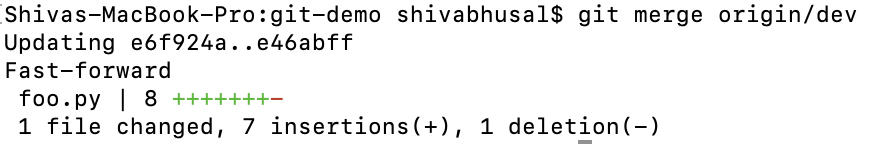
\includegraphics[scale=0.85]{figure/merge.png}}
    \caption{\textit{git merge} operation}
  \end{figure}

\subsection{git log}
It displays the version history of the repository or the list of the historical commits. 
\begin{lstlisting}[language=Bash]
git log
\end{lstlisting}

\section{Using .gitignore}
It is not a good practice to push binary files, log files, and executable. You may also want to exclude some directories of the project from being pushed. In order to exclude the selective files and directories, a \textit{.gitignore} file can be used.To learn more about it,  refer to the official \href{https://git-scm.com/docs/gitignore}{\textit{Git} Documentation}

\end{document}

%%% End of our document 